\documentclass[11pt]{article}
\usepackage[a4paper,margin=21mm]{geometry}
\usepackage{fontspec}
\setmainfont{Latin Modern Roman}
\newfontfamily\CJKfont{Noto Serif CJK SC}
\XeTeXlinebreaklocale "zh"
\XeTeXlinebreakskip=0pt plus 1pt
\usepackage{amsmath,amssymb,amsthm,amscd,graphicx,color}
\usepackage{xurl}
\usepackage[unicode,hidelinks]{hyperref}
\allowdisplaybreaks
\setlength\emergencystretch{3em}
\numberwithin{equation}{section}
\newtheorem*{Theorem*}{Theorem}
\newtheorem{Theorem}{Theorem}[section]
\newtheorem{Corollary}[Theorem]{Corollary}
\newtheorem{Lemma}[Theorem]{Lemma}
\newtheorem{Proposition}[Theorem]{Proposition}
\newtheorem{Claim}[Theorem]{Claim}
 { \theoremstyle{definition}
\newtheorem{Definition}[Theorem]{Definition}
\newtheorem{Note}[Theorem]{Note}
\newtheorem{Example}[Theorem]{Example}
\newtheorem{Remark}[Theorem]{Remark}
\newtheorem{Problem}[Theorem]{Problem}
}

\newcommand{\R}{\mathbb{R}} %real numbers
\newcommand{\Q}{\mathbb{Q}} %rational numbers
\newcommand{\C}{\mathbb{C}} % complex numberse
\newcommand{\Z}{\mathbb{Z}} %integers
\newcommand{\N}{\mathbb{N}} % the natural numbers
\newcommand{\h}{\mathbb{H}} % upper half plane

\newcommand{\SL}{\mathrm{SL}}

\newcommand{\sage}{\texttt{sage} }

\newcommand{\bs}{\backslash}

\newcommand{\calA}{\mathcal{A}}
\newcommand{\calB}{\mathcal{B}}
\newcommand{\calC}{\mathcal{C}}
\newcommand{\calD}{\mathcal{D}}
\newcommand{\calE}{\mathcal{E}}
\newcommand{\calF}{\mathcal{F}}
%\newcommand{\F}{\mathcal{F}}
\newcommand{\calG}{\mathcal{G}}
\newcommand{\calH}{\mathcal{H}}
\newcommand{\calI}{\mathcal{I}}
\newcommand{\calJ}{\mathcal{J}}
\newcommand{\calK}{\mathcal{K}}
\newcommand{\calL}{\mathcal{L}}
%\newcommand{\calM}{\mathcal{M}}
\newcommand{\M}{\mathcal{M}}
\newcommand{\calN}{\mathcal{N}}
\newcommand{\calO}{\mathcal{O}}
\newcommand{\calP}{\mathcal{P}}
\newcommand{\calQ}{\mathcal{Q}}
\newcommand{\calR}{\mathcal{R}}
\newcommand{\calS}{\mathcal{S}}
\newcommand{\calT}{\mathcal{T}}
\newcommand{\calV}{\mathcal{V}}
\newcommand{\calW}{\mathcal{W}}
\newcommand{\calX}{\mathcal{X}}
\newcommand{\calY}{\mathcal{Y}}
\newcommand{\calZ}{\mathcal{Z}}

\newcommand{\frakA}{\mathfrak{A}}
\newcommand{\fraka}{\mathfrak{a}}
\newcommand{\frakb}{\mathfrak{b}}
\newcommand{\frakc}{\mathfrak{c}}
\newcommand{\frakd}{\mathfrak{d}}
\newcommand{\frake}{\mathfrak{e}}
\newcommand{\frakE}{\mathfrak{E}}
\newcommand{\frakF}{\mathfrak{F}}
\newcommand{\frakf}{\mathfrak{f}}
\newcommand{\frakg}{\mathfrak{g}}
\newcommand{\frakG}{\mathfrak{G}}
\newcommand{\efrak}{\mathfrak{e}}
\newcommand{\frakN}{\mathfrak{N}}
\newcommand{\frakm}{\mathfrak{m}}
\newcommand{\frakn}{\mathfrak{n}}
\newcommand{\frakp}{\mathfrak{p}}
\newcommand{\frakP}{\mathfrak{P}}
\newcommand{\frakQ}{\mathfrak{Q}}
\newcommand{\frakt}{\mathfrak{t}}
\newcommand{\frakT}{\mathfrak{T}}

\def\({\left(}
\def\){\right)}
\def\ddd{{\rm d}}

\def\lp{\left(}
\def\rp{\right)}
\def\lb{\left[}
\def\rb{\right]}

\renewcommand{\textfraction}{0.01}
\renewcommand{\topfraction}{0.99}

\begin{document}
\begin{center}\Large Uniform asymptotics of hook polynomials outside the unit annulus\end{center}
\noindent\textbf{Stable ID:} 558\quad\textbf{Author:} Walter Bridges; William Craig; Amanda Folsom; Larry Rolen\par
\noindent\textbf{Work:} Zeros of Hook Polynomials and Related Questions\par
\noindent\textbf{Source:} \url{https://sigma-journal.com/2025/026/}\par
\noindent\textbf{Version:} Official SIGMA 21 (2025) PDF and native TeX; acquired 2026-09-30; exact bytes pinned by SHA256\par
\noindent\textbf{Rights:} CC BY 4.0. Authors retain copyright. \url{https://creativecommons.org/licenses/by/4.0/}. Reuse and typesetting adaptation; original language and mathematical content preserved.\par
\noindent\textbf{Difficulty (prior selection preserved):} {\CJKfont H2: The circle-method decomposition must remain uniform in a complex polynomial parameter, separate all root-of-unity arcs, and prevent cancellation of the dominant theta factor. The nonzero-theta exclusion and minor-arc controls are essential beyond merely applying Laplace’s method to the final saddle integral.}\par
\medskip\noindent\textbf{Editorial boundary note (not author text):} Complete original Theorem 1.2 and full Farey-arc/modular-transform/saddle calculation for the large-w residue-class asymptotic. Retains exact hook-polynomial/generating-function/theta/excluded-zero notation, the author-cited Han product and Laplace-method prerequisites, minor-arc estimate, main-arc transformation, error bound and full constant. The numerical Young-hook illustration alone is copied from the unchanged original PDF as a small vector figure because ytableau is unavailable; all statement and proof mathematics remains editable native TeX. The separate small-w theorem and polynomial-zero plots are excluded.\par
\medskip\hrule\medskip\noindent\textbf{Author text begins below.}\par
\setcounter{section}{1}
% Original source lines 156--165
For a positive integer $n$, a {\it partition} of $n$ is a non-increasing sequence $\lambda = \lp \lambda_1, \dots, \lambda_\ell \rp$ of positive integers such that $|\lambda| := \lambda_1 + \dots + \lambda_\ell = n$. We write $\lambda \vdash n$ to denote that $\lambda$ is a partition of $n$, and we let $\ell = \ell\lp \lambda \rp$ be the number of parts of $\lambda$. Since the very beginning of partition theory, generating functions have been an essential tool. In the last century, the {\it circle method}
as developed first by Hardy and Ramanujan \cite{HR} has become an indispensable tool in studying the coefficients of these generating functions as well as many counting problems in additive combinatorics and number theory, including the Waring problem and weak Goldbach conjecture. Hardy and Ramanujan used the generating function for the {\it partition function} $p(n) := \#\{ \lambda \vdash n \}$, given for $|q|<1$ by
\begin{align*}
 \sum_{n \geq 0} p(n) q^n = \prod_{n \geq 1} \dfrac{1}{1 - q^n},
\end{align*}
in order to prove an asymptotic series for $p(n)$ as $n \to \infty$, whose main term yields
\begin{align*}
 p(n) \sim \dfrac{1}{4n\sqrt{3}} {\rm e}^{\pi\sqrt{\frac{2n}{3}}}.
\end{align*}



% Original source lines 181--201
In this paper, we will approach a problem of two of the authors and Males \cite{FMR} on {\it hook polynomials} which arose in their study of the connection between zeros of partition polynomials and crank statistics. In order to explain the problem, we require hook numbers of partitions. For each cell of the Young diagram of a partition $\lambda$, the {\it hook number} of this cell is the number of boxes that form the inverted $L$-shape whose corner resides at the cell in question. For instance, the hook numbers of the partition $\lambda = \lp 5, 2, 1 \rp$ are given as
\begin{figure}[ht]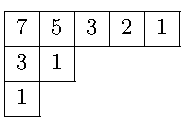
\includegraphics[width=89bp]{../assets/558/original-hook-tableau.pdf}\end{figure}

 We let $\mathcal H(\lambda)$ be the multiset of all hook numbers of $\lambda$ and the $t$-hook multiset as
\begin{align*}
 \mathcal H_t(\lambda) := \{ h \in \mathcal H(\lambda) : t \mid h \}.
\end{align*}
In order to keep track of the number of $t$-hooks of partitions, we use a formula for the generating function due to Han, which derives from his extensions of the Nekrasov--Okounkov hook lengths formula \cite{Han,NekOk}. To state this theorem and those that follow, we define for each $t \geq 1$ the generating functions
\begin{align*}
 H_t\lp w;q \rp := \sum_{n \geq 0} P_t(w;n) q^n := \sum_{\lambda} w^{\#\mathcal H_t(\lambda)} q^{|\lambda|} .
\end{align*}

The following representation for $H_t(w;q)$ is proven in \cite[Corollary 5.1]{Han}.

\begin{Theorem}
 We have for $t \geq 2$ that
 \begin{align*}
 H_t(w;q) = \prod_{n \geq 1} \frac{1}{(1-(wq^t)^n)^t}\prod_{n \geq 1} \frac{\big(1-q^{tn}\big)^t}{1-q^n}.
 \end{align*}
\end{Theorem}


% Original source lines 223--238
 To state the asymptotics for $P_t(w,n)$ in the case $|w|>1$, we define, for $|z|<1$, the theta function
\begin{align*}
 \Theta_{\ell,t}(z):=\sum_{\substack{\boldsymbol{m}\in \mathbb{Z}^t \\ \boldsymbol{1} \cdot \boldsymbol{m}=0 \\ \boldsymbol{b}\cdot \boldsymbol{m} \equiv \ell \ ({\text{mod}\, {t}}) }} z^{\frac{1}{2}\|\boldsymbol{m}\|^2+\frac{1}{t}\boldsymbol{b}\cdot \boldsymbol{m}},
\end{align*} where $\boldsymbol{b}:=(0,1,\dots,t-1)$. For $\epsilon>0$, let
\begin{align*}
\mathcal{Z}_{\ell,t}(\epsilon):=\bigl\{z : |z|\geq 1+\epsilon, \, \Theta_{\ell,t}\big(z^{-1}\big)=0\bigr\}.
\end{align*}
Since $\Theta_{\ell,t}(z)$ is analytic and nonzero in $|z|<1$, it follows that $\#\mathcal{Z}_{\ell,t}(\epsilon)<\infty$ for all $\epsilon>0$.

\begin{Theorem} \label{|w|>1 Asymptotics}
 Let $t
 \geq 1$ and let $\epsilon>0$. Then uniformly for $|w|>1+\epsilon$ and $w$ not in an $\epsilon$-neighborhood of $\mathcal{Z}_{\ell,t}(\epsilon)$, we have, as $n \to \infty$ along the residue class $\ell \pmod{t}$,
 \begin{align*}
P_t(w,n)= {\rm e}^{\pi \sqrt{\frac{2n}{3}}}w^{\frac{n}{t}} \Theta_{\ell,t}\big(w^{-1}\big)\frac{1}{2^{\frac{5+t}{4}}3^{\frac{1+t}{4}}\pi^{\frac{3+t}{2}}n^{\frac{3+t}{4}}}(1+o(1)).
 \end{align*}
\end{Theorem}


% Original source lines 264--385
\section{Asymptotics for hook-length polynomials} \label{S: Asymptotics}

\subsection[The case |w|>1]{The case $\boldsymbol{|w|>1}$} %\label{S:smallw}

Throughout this section, we use the abbreviated $q$-Pochhammer,
\begin{align*}
(a)_{\infty}:=(a;a)_{\infty}=\prod_{k \geq 1} \big(1-a^k\big).
\end{align*}
Note that by \cite[equation~(3.1)]{GKS}, we may rewrite
\begin{align*}
 \Theta_{\ell,t}(z)&{}=\sum_{\substack{\boldsymbol{m}\in \mathbb{Z}^t \\ \boldsymbol{1} \cdot \boldsymbol{m}=0 \\ \boldsymbol{b}\cdot \boldsymbol{m} \equiv \ell \ (\text{mod}\, {t}) }} \! z^{\frac{1}{2}\|\boldsymbol{m}\|^2+\frac{1}{t}\boldsymbol{b}\cdot \boldsymbol{m}}
 = (z)_{\infty}^t \sum_{\substack{m \geq 0 \\ m \equiv \ell \ (\text{mod}\, {t})}}\! p(m)z^{\frac{m}{t}}
=\frac{1}{t}\sum_{j=0}^{ t-1}{\rm e}^{-2\pi {\rm i} \frac{j\ell}{t}}\frac{(z)_{\infty}^t}{\big(z^{\frac{1}{t}}{\rm e}^{2\pi {\rm i} \frac{j}{t}}\big)_{\infty}}.
\end{align*}
It is in the latter form that $\Theta_{\ell,t}$ will appear in the proof of Theorem \ref{|w|>1 Asymptotics}. We will also make use of the version of Laplace's Method below that is sufficient for our purposes.
\begin{Theorem}[Laplace's method, see {\cite[Section 1.1.5]{Pinsky}}]\label{T:LaplaceMethod}
 Let $A,B\colon [a,b]\to \mathbb{C}$ be continuous functions. Let $x_0 \in (a,b)$ and suppose $\mathrm{Re}(B(x))<\mathrm{Re}(B(x_0))$ for all $x\in (a,b)$ with $x \neq x_0$. Suppose further that
 \begin{align*}
 \lim_{x\to x_0}\frac{B(x)-B(x_0)}{(x-x_0)^2} = -k\in \mathbb{C},
 \end{align*}
 with $\mathrm{Re}(k)>0.$ Then as $t \to \infty$,
 \begin{align*}
 \int^b_{a}A(x){\rm e}^{tB(x)}{\rm d}x = {\rm e}^{tB(x_0)}\biggl(A(x_0)\sqrt{\frac{\pi}{tk}}+o\biggl(\frac{1}{\sqrt{t}}\biggr)\biggr).
 \end{align*}
\end{Theorem}

We are now ready to prove Theorem \ref{|w|>1 Asymptotics}.


\begin{proof}[Proof of Theorem \ref{|w|>1 Asymptotics}] If $|w|>1$, then $P_t(w,q)$ is analytic in the region
 \begin{align*}
 \bigl|wq^t\bigr|<1 \ \iff\  |q|< |w|^{-\frac{1}{t}}<1.
 \end{align*}
 Now, let \smash{$x_n:= \frac{\pi}{\sqrt{6n}} \to 0^+$}. Choose a $t$-th root of $w$. Then
 \begin{align*}
 P_t(w,n)&{}=\frac{1}{2\pi {\rm i}} \int_{\substack{q=w^{-\frac{1}{t}}{\rm e}^{-x_n+2\pi {\rm i} \theta} \\ |\theta|\leq \frac{1}{2}}} \frac{H_t(w;q)}{q^{n+1}} \,{\rm d}q \\
 &{}={\rm e}^{nx_n}w^{\frac{n}{t}}\int_{|\theta|\leq \frac{1}{2}} H_t\big(w;w^{-\frac{1}{t}}{\rm e}^{-x_n+2\pi {\rm i} \theta}\big){\rm e}^{-2\pi {\rm i} n \theta} {\rm d}\theta \\
 &{}={\rm e}^{nx_n}w^{\frac{n}{t}}\int_{|\theta|\leq \frac{1}{2}} \big({\rm e}^{-tx_n+2\pi {\rm i} t \theta}\big)_{\infty}^{-t}\frac{\big(w^{-1}{\rm e}^{-tx_n+2\pi {\rm i} t \theta}\big)_{\infty}^t}{\big(w^{-\frac{1}{t}}{\rm e}^{-x_n+2\pi {\rm i} \theta}\big)_{\infty}}{\rm e}^{-2\pi {\rm i} n \theta} {\rm d}\theta.
 \end{align*}
 Now set \smash{$\theta\mapsto \frac{1}{t}(\theta+j)$} for $0\leq j \leq t-1$. Then we obtain
 \begin{align*}
 P_t(w,n)
 =\frac{{\rm e}^{nx_n}w^{\frac{n}{t}}}{t}\sum_{j=0}^{ t-1}{\rm e}^{-2\pi {\rm i} \frac{jn}{t}}\int_{|\theta|\leq \frac{1}{2}} \big({\rm e}^{-tx_n+2\pi {\rm i} \theta}\big)_{\infty}^{-t}\frac{\big(w^{-1}{\rm e}^{-tx_n+2\pi {\rm i} \theta}\big)_{\infty}^t}{\big(w^{-\frac{1}{t}}{\rm e}^{2\pi {\rm i} \frac{j}{t}-x_n+2\pi {\rm i} \frac{\theta}{t}}\big)_{\infty}}{\rm e}^{-2\pi {\rm i} \frac{n}{t} \theta} {\rm d}\theta.
 \end{align*}
 Let $\mathcal{F}_N$ be the Farey sequence of order $N$ (to be chosen later in the proof) and $\theta_{h,k}'$, $\theta_{h,k}''$ the respective mediants of three consecutive fractions $\frac{h'}{k'},\frac{h}{k},\frac{h''}{k''} \in \mathcal{F}_N$. Then
 \begin{align*}
 P_t(w,n)
 &{}=\frac{{\rm e}^{nx_n}w^{\frac{n}{t}}}{t}\sum_{j=0}^{ t-1}{\rm e}^{-2\pi {\rm i} \frac{jn}{t}} \sum_{\frac{h}{k} \in \mathcal{F}_N} {\rm e}^{-2\pi {\rm i} \frac{hn}{kt}} \\
 &\hphantom{=\frac{{\rm e}^{nx_n}w^{\frac{n}{t}}}{t}\sum_{j=0}^{ t-1}}\,{} \times \int_{-\theta_{h,k}'}^{\theta_{h,k}''} \!\big({\rm e}^{-tx_n+2\pi {\rm i} \theta+2\pi {\rm i} \frac{h}{k}}\big)_{\infty}^{-t}\frac{\big(w^{-1}{\rm e}^{-tx_n+2\pi {\rm i} \theta+2\pi {\rm i} \frac{h}{k}}\big)_{\infty}^t}{(w^{-\frac{1}{t}}{\rm e}^{2\pi {\rm i} \frac{j}{t}-x_n+2\pi {\rm i} \frac{\theta}{t}+2\pi {\rm i} \frac{h}{kt}})_{\infty}}{\rm e}^{-2\pi {\rm i} \frac{n}{t} \theta} {\rm d}\theta.
 \end{align*}
 Since the middle factor of the integrand is analytic for $|q|=1$, we have, as $x_n \to 0^+$,
 \begin{align}
 \frac{\big(w^{-1}{\rm e}^{-tx_n+2\pi {\rm i} \theta+2\pi {\rm i} \frac{h}{k}}\big)_{\infty}^t}{\big(w^{-\frac{1}{t}}{\rm e}^{2\pi {\rm i} \frac{j}{t}-x_n+2\pi {\rm i} \frac{\theta}{t}+2\pi {\rm i} \frac{h}{kt}}\big)_{\infty}} =\frac{\big(w^{-1}{\rm e}^{2\pi {\rm i} \frac{h}{k}}\big)_{\infty}^t}{\big(w^{-\frac{1}{t}}{\rm e}^{2\pi {\rm i} \frac{j}{t}+2\pi {\rm i} \frac{h}{kt}}\big)_{\infty}}(1+x_n E_{j,h,k,t,n,w}(\theta)), \label{E:Ejhktw}
 \end{align}
 where $E_{j,h,k,t,n,w}(\theta)$ is a continuous function of $\theta$, uniformly bounded with respect to~$j$,~$h$,~$k$,~$n$ and for $|w|\geq 1+\epsilon$. Set $N:=\lfloor \sqrt{n} \rfloor$.
 Here, $\theta_{h,k}',\theta_{h,k}'' \asymp \frac{1}{kN} \to 0$ \cite[p.~75]{Andrews}. Thus, using the continuity of the above function of $\theta$,
 \begin{align*}
 P_t(w,n)
 &{}=\frac{{\rm e}^{nx_n}w^{\frac{n}{t}}}{t}\sum_{j=0}^{ t-1}{\rm e}^{-2\pi {\rm i} \frac{jn}{t}} \sum_{\frac{h}{k} \in \mathcal{F}_N} {\rm e}^{-2\pi {\rm i} \frac{hn}{kt}}\frac{\big(w^{-1}{\rm e}^{2\pi {\rm i} \frac{h}{k}}\big)_{\infty}^t}{\big(w^{-\frac{1}{t}}{\rm e}^{2\pi {\rm i} \frac{j}{t}+2\pi {\rm i} \frac{h}{kt}}\big)_{\infty}} \\[-1mm]
 &\hphantom{=\frac{{\rm e}^{nx_n}w^{\frac{n}{t}}}{t}\sum_{j=0}^{ t-1}}\,{} \times \int_{-\theta_{h,k}'}^{\theta_{h,k}''} \big({\rm e}^{-tx_n+2\pi {\rm i} \theta+2\pi {\rm i} \frac{h}{k}}\big)_{\infty}^{-t}{\rm e}^{-2\pi {\rm i} \frac{n}{t} \theta}(1+x_n E_{j,h,k,n,t,w}(\theta)) \,{\rm d}\theta \\[-1mm]
 &{}={\rm e}^{nx_n}w^{\frac{n}{t}} \sum_{\frac{h}{k} \in \mathcal{F}_N} {\rm e}^{-2\pi {\rm i} \frac{hn}{kt}}\Theta_{n,t}\big(w^{-1}{\rm e}^{2\pi {\rm i} \frac{h}{k}}\big) \\[-1mm]
 &\hphantom{={\rm e}^{nx_n}w^{\frac{n}{t}} \sum_{\frac{h}{k} \in \mathcal{F}_N}}\,{} \times \int_{-\theta_{h,k}'}^{\theta_{h,k}''} \big({\rm e}^{-tx_n+2\pi {\rm i} \theta+2\pi {\rm i} \frac{h}{k}}\big)_{\infty}^{-t}{\rm e}^{-2\pi {\rm i} \frac{n}{t} \theta}(1+x_n E_{j,h,k,n,t,w}(\theta)) \,{\rm d}\theta.
 \end{align*}

 Note that $\Theta_{n,t}\big(w^{-1}{\rm e}^{2\pi {\rm i} \frac{h}{k}}\big)=\Theta_{\ell,t}\big(w^{-1}{\rm e}^{2\pi {\rm i} \frac{h}{k}}\big)$ is uniformly bounded for all $\frac{h}{k} \in \mathcal{F}_N$ and all $|w|>1+\epsilon$, so does not contribute to asymptotic growth. Now, by \cite[equation~(5.2.2)]{Andrews}, with
 \begin{align*}
 2\pi {\rm i} \frac{h+{\rm i}z}{k}=-tx_n+2\pi {\rm i} \theta+2\pi {\rm i} \frac{h}{k} \ \implies\  z=\frac{ktx_n}{2\pi}-k{\rm i}\theta,
 \end{align*}
 and $hh' \equiv -1 \pmod{k}$ and $\omega_{h,k}={\rm e}^{\pi {\rm i} s(h,k)}$, where $s(h,k)$ is the Dedekind sum as in \cite[equation~(5.2.4)]{Andrews},
\begin{align*}
 &\big({\rm e}^{-tx_n+2\pi {\rm i} \theta+2\pi {\rm i} \frac{h}{k}}\big)_{\infty}^{-t} \\[-1mm]
 &{}= \omega_{h,k}^t \biggl(\frac{ktx_n}{2\pi}-k{\rm i}\theta\biggr)^{\frac{t}{2}}{\rm e}^{\frac{\pi t}{12k(\frac{ktx_n}{2\pi}-k{\rm i}\theta)}-\pi t\frac{\frac{ktx_n}{2\pi}-k{\rm i}\theta}{12k}}\Biggl(1+O\Biggl( {\rm e}^{2\pi {\rm i}\frac{h'+\frac{{\rm i}}{\frac{ktx_n}{2\pi}-k{\rm i}\theta}}{k}}\Biggr) \Biggr) \\[-1mm]
 &{}= \omega_{h,k}^t k^{\frac{t}{2}} \biggl(\frac{tx_n}{2\pi}-{\rm i}\theta\biggr)^{\frac{t}{2}}{\rm e}^{\frac{\pi t}{12}\big(\frac{1}{k^2(\frac{tx_n}{2\pi}-{\rm i}\theta)}-(\frac{tx_n}{2\pi}-{\rm i}\theta)\big)}\Biggl(1+\Biggl( {\rm e}^{- \frac{2\pi}{1+(\frac{2\pi\theta}{tx_n})^2}}\Biggr) \Biggr) \\[-1mm]
 &{}= \omega_{h,k}^t k^{\frac{t}{2}} \biggl(\frac{tx_n}{2\pi}-{\rm i}\theta\biggr)^{\frac{t}{2}}{\rm e}^{\frac{\pi t}{12k^2(\frac{tx_n}{2\pi}-{\rm i}\theta)}}(1+O(x_n)) \biggl(1+O\biggl(\frac{1}{kN}\biggr) \biggr) \Biggl(1+O\Biggl( \frac{1}{1+\frac{1}{(tx_nkN)^2}}\Biggr) \Biggr).
\end{align*}
Thus,
 \begin{align}
 P_t(w,n) &{}={\rm e}^{nx_n}w^{\frac{n}{t}} \sum_{\frac{h}{k} \in \mathcal{F}_{\lfloor \sqrt{n} \rfloor}} \omega_{h,k}^tk^{\frac{t}{2}}{\rm e}^{-2\pi {\rm i} \frac{hn}{kt}}\Theta_{\ell,t}\big(w^{-1}{\rm e}^{2\pi {\rm i} \frac{h}{k}}\big)(1+o(1)) \label{E:CircleMethodSeries}\\[-1mm]
 &\hphantom{={\rm e}^{nx_n}w^{\frac{n}{t}} \sum_{\frac{h}{k} \in \mathcal{F}_{\lfloor \sqrt{n} \rfloor}}}{}
 \times \int_{-\theta_{h,k}'}^{\theta_{h,k}''} \! \biggl(\frac{tx_n}{2\pi}-{\rm i}\theta\biggr)^{\frac{t}{2}}\!{\rm e}^{\frac{\pi t}{12k^2(\frac{tx_n}{2\pi}-{\rm i}\theta)}-2\pi {\rm i} \frac{n}{t} \theta}\! (1+x_n E_{j,h,k,t,n,w}(\theta))\, {\rm d}\theta, \nonumber
 \end{align}
and we are left to bound the integrals. Choose $N:=\lfloor \sqrt{n} \rfloor$, so that for $k \geq 2$,{\samepage
\begin{align*}
 & \biggl|
 \int_{-\theta_{h,k}'}^{\theta_{h,k}''} \biggl(\frac{tx_n}{2\pi}-{\rm i}\theta\biggr)^{\frac{t}{2}}{\rm e}^{\frac{\pi t}{12k^2(\frac{tx_n}{2\pi}-{\rm i}\theta)}-2\pi {\rm i} \frac{n}{t} \theta} (1+x_n E_{j,h,k,n,t,w}(\theta)) \,{\rm d}\theta \biggr| \\[-1mm]
 &\qquad{} \ll \int_{-\theta_{h,k}'}^{\theta_{h,k}''} \biggl|\frac{tx_n}{2\pi}-{\rm i}\theta \biggr|^{\frac{t}{2}} {\rm e}^{\frac{\pi t \cdot \frac{tx_n}{2\pi}}{12k^2(\frac{t^2x_n^2}{4\pi^2}+\theta^2)}} {\rm d}\theta
 \ll \frac{1}{kN}{\rm e}^{\frac{\pi^2}{6k^2x_n}}
 =o\Bigl({\rm e}^{\frac{\pi^2}{6x_n}}\Bigr),
\end{align*}
where we used the boundedness of $E_{j,h,k,n,t,w}(\theta)$.}

For $k=1$, we have $\theta_{0,1}'=\theta_{0,1}''=\frac{1}{N+1}$ and we apply Theorem \ref{T:LaplaceMethod}.
We first need to transform the integral to be of the correct form. We first set $\theta \mapsto \theta \frac{tx_n}{2\pi}$. Thus,
\begin{align}
 &\int_{-\frac{1}{N+1}}^{\frac{1}{N+1}} \biggl(\frac{tx_n}{2\pi}-{\rm i}\theta\biggr)^{\frac{t}{2}}{\rm e}^{\frac{\pi t}{12(\frac{tx_n}{2\pi}-{\rm i}\theta)}-2\pi {\rm i} \frac{n}{t} \theta} (1+x_n E_{j,0,1,n,t,w}(\theta)) \,{\rm d}\theta \nonumber \\
 &\qquad{}=\frac{tx_n}{2\pi}\int_{-\frac{2\pi}{tx_n(N+1)}}^{\frac{2\pi}{tx_n(N+1)}} \biggl(\frac{tx_n}{2\pi}-\frac{{\rm i}tx_n\theta}{2\pi}\biggr)^{\frac{t}{2}}{\rm e}^{\frac{\pi}{12(\frac{x_n}{2\pi}-\frac{{\rm i}x_n\theta}{2\pi})}- {\rm i} nx_n \theta} \biggl(1+x_n E_{j,0,1,n,t,w}\biggl(\frac{tx_n\theta}{2\pi}\biggr)\biggr) {\rm d}\theta \nonumber \\
 &\qquad{}=\frac{t^{\frac{t+2}{2}}x_n^{\frac{t+2}{2}}}{(2\pi)^{\frac{t+2}{2}}}\int_{-\frac{2\pi}{tx_n(N+1)}}^{\frac{2\pi}{tx_n(N+1)}} (1-{\rm i}\theta)^{\frac{t}{2}}{\rm e}^{\frac{\pi^2}{6x_n}( \frac{1}{1-{\rm i}\theta}- {\rm i} \theta)} \biggl(1+x_n E_{j,0,1,n,t,w}\biggl(\frac{tx_n\theta}{2\pi}\biggr)\biggr) {\rm d}\theta. \label{E:MainRewrite}
\end{align}
Now, as \smash{$x_n, \frac{1}{N+1} \asymp \frac{1}{\sqrt{n}}$}, it follows that the bounds of the integral above are bounded away from~0 and~$\infty$ and are of the form needed for Theorem \ref{T:LaplaceMethod}. We would like to apply Theorem \ref{T:LaplaceMethod} with $x\mapsto \theta$, $x_0\mapsto 0$, \smash{$A(\theta)=(1-{\rm i}\theta)^{\frac{1}{2}}$} and $B(\theta)=\frac{1}{1-{\rm i}\theta}- {\rm i} \theta$. Here,
\begin{align*}
 \mathrm{Re} \lp B(\theta) \rp = \frac{1}{1+\theta^2}< 1
\end{align*}
for $\theta \neq 0$ and Taylor expanding gives
\begin{align*}
 B(\theta)=1-\theta^2+O\big(\theta^3\big).
\end{align*}
First we bound the error term, using the boundedness of $E_{j,0,1,n,t,w}$, as
\begin{equation}\label{E:MainTerm}
\biggl|\int_{-\frac{2\pi}{tx_n(N+1)}}^{\frac{2\pi}{tx_n(N+1)}} (1-{\rm i}\theta)^{\frac{t}{2}}{\rm e}^{\frac{\pi^2}{6x_n}( \frac{1}{1-{\rm i}\theta}- {\rm i}\theta)} x_n E_{j,0,1,n,t,w}\biggl(\frac{tx_n\theta}{2\pi}\biggr) {\rm d}\theta \biggr| \ll {\rm e}^{\frac{\pi^2}{6x_n}}x_n.
\end{equation}
For the main term, Theorem \ref{T:LaplaceMethod} gives
\begin{equation}\label{E:MainError}
\int_{-\frac{2\pi}{tx_n(N+1)}}^{\frac{2\pi}{tx_n(N+1)}} (1-{\rm i}\theta)^{\frac{t}{2}}{\rm e}^{\frac{\pi^2}{6x_n}( \frac{1}{1-{\rm i}\theta}- {\rm i}\theta)}={\rm e}^{\frac{\pi^2}{6x_n}}\Biggl(\sqrt{\frac{\pi6x_n}{\pi^2}}+o\big( \sqrt{x_n}\big)\Biggr),
\end{equation}
hence \eqref{E:MainRewrite}--\eqref{E:MainError} imply
\begin{align}
 \int_{-\frac{1}{N+1}}^{\frac{1}{N+1}} \biggl(\frac{tx_n}{2\pi}-{\rm i}\theta\biggr)^{\frac{t}{2}}{\rm e}^{\frac{\pi t}{12(\frac{tx_n}{2\pi}-{\rm i}\theta)}-2\pi {\rm i} \frac{n}{t} \theta} {\rm d}\theta
 &{}=\frac{t^{\frac{2+t}{2}}x_n^{\frac{2+t}{2}}}{(2\pi)^{\frac{2+t}{2}}}{\rm e}^{\frac{\pi^2}{6x_n}}\Biggl(\sqrt{\frac{\pi6x_n}{\pi^2}}+o( 1) \Biggr) \nonumber \\
 &{}=\frac{1}{2^{\frac{5+t}{4}}3^{\frac{1+t}{4}}\pi^{\frac{3+t}{2}}n^{\frac{3+t}{4}}}{\rm e}^{\frac{\pi\sqrt{n}}{\sqrt{6}}}(1+o(1)). \label{E:wlargemainterm}
\end{align}
Since we assume that $w^{-1}$ is not in an $\epsilon$-neighborhood of $\mathcal{Z}_{\ell,t}(\epsilon)$, it follows that the main term in \eqref{E:CircleMethodSeries} does not vanish and occurs for $k=1$. Combining with \eqref{E:wlargemainterm} and using $\omega_{0,1}=1$, the theorem follows.
\end{proof}
\begin{thebibliography}{99}
\bibitem[2]{Andrews}
Andrews G.E., The theory of partitions, \textit{Cambridge Math. Lib.}, \href{https://doi.org/10.1017/CBO9780511608650}{Cambridge
 University Press}, Cambridge, 1984.

\bibitem[13]{FMR}
Folsom A., Males J., Rolen L., Equidistribution and partition polynomials,
 \href{https://doi.org/10.1007/s11139-023-00762-w}{\textit{Ramanujan~J.}} \textbf{65} (2024), 1827--1848, \href{https://arxiv.org/abs/2209.15114}{arXiv:2209.15114}.

\bibitem[15]{GKS}
Garvan F., Kim D., Stanton D., Cranks and {$t$}-cores, \href{https://doi.org/10.1007/BF01231493}{\textit{Invent. Math.}}
 \textbf{101} (1990), 1--17.

\bibitem[18]{Han}
Han G.N., The {N}ekrasov--{O}kounkov hook length formula: refinement,
 elementary proof, extension and applications, \href{https://doi.org/10.5802/aif.2515}{\textit{Ann. Inst. Fourier
 (Grenoble)}} \textbf{60} (2010), 1--29, \href{https://arxiv.org/abs/0805.1398}{arXiv:0805.1398}.

\bibitem[19]{HR}
Hardy G.H., Ramanujan S., Asymptotic formulaae in combinatory analysis,
 \href{https://doi.org/10.1112/plms/s2-17.1.75}{\textit{Proc. London Math. Soc.}} \textbf{17} (1918), 75--115.

\bibitem[28]{NekOk}
Nekrasov N.A., Okounkov A., Seiberg--{W}itten theory and random partitions, in
 The Unity of Mathematics, \textit{Progr. Math.}, Vol. 244, \href{https://doi.org/10.1007/0-8176-4467-9_15}{Birkh\"auser},
 Boston, MA, 2006, 525--596, \href{https://arxiv.org/abs/hep-th/0306238}{arXiv:hep-th/0306238}.

\bibitem[30]{Pinsky}
Pinsky M.A., Introduction to {F}ourier analysis and wavelets, \textit{Grad.
 Stud. Math.}, Vol. 102, \href{https://doi.org/10.1090/gsm/102}{American Mathematical Society}, Providence, RI, 2009.

\end{thebibliography}
\end{document}
